\subsection{Historia y evolución del estándar Fibre Channel}

Fibre Channel fue desarrollado a principios de los años 1990 como un estándar unificado que combinaba las mejores características de las tecnologías existentes en ese momento, incluyendo SCSI, Fibre Optic Channel y otras tecnologías de red. El objetivo era crear un protocolo de alta velocidad que pudiera manejar tanto almacenamiento como comunicaciones de red, aunque finalmente se especializó predominantemente en almacenamiento. La primera versión de la tecnología, el 1G FC, fue introducida en 1997, proporcionando una tasa de transferencia de 200 Megabytes por segundo. Esta versión inicial estableció las bases para todas las evoluciones posteriores y demostró la viabilidad de la tecnología para entornos empresariales.

La evolución de las velocidades de Fibre Channel ha sido constante y predecible. El 2G FC fue lanzado en 2001, duplicando la velocidad a 2.125 Gbps. El 4G FC llegó en 2004, alcanzando 4.25 Gbps. El 8G FC fue introducido en 2007, proporcionando 8.5 Gbps. El 16G FC apareció en 2011, oferendo 16.125 Gbps. El 32G FC fue lanzado alrededor de 2016, proporcionando 32.25 Gbps. Se han desarrollado estándares de 64G FC y 128G FC, aunque estos últimos se implementan comúnmente mediante multiplexación por división de longitud de onda (DWDM) de múltiples canales de 32G en lugar de velocidades de señal individuales más altas.

Cada generación de Fibre Channel ha mantenido retrocompatibilidad completa con versiones anteriores, lo que permite que dispositivos de diferentes velocidades coexistan en la misma red. Esta característica ha sido fundamental para la adopción y longevidad de la tecnología, permitiendo a las organizaciones actualizar gradualmente su infraestructura sin reemplazar completamente los equipos existentes.

\subsection{Capas del protocolo Fibre Channel: FC-0 a FC-4}

El protocolo Fibre Channel utiliza una arquitectura de cinco capas numeradas de FC-0 a FC-4, cada una con funciones específicas que trabajan en conjunto para proporcionar comunicación confiable de alta velocidad.

\begin{figure}[H]
	\centering
	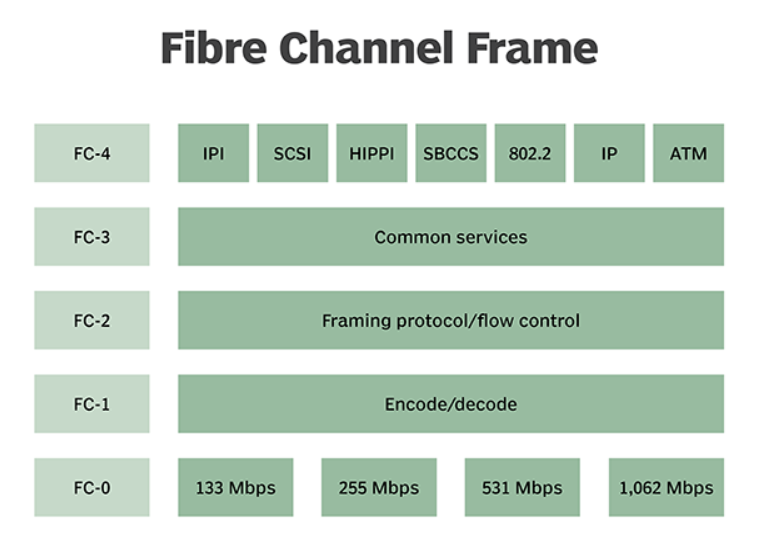
\includegraphics[width=0.5\textwidth]{img/san4.png}
	\caption{Capas Canal de Fibra}
	\label{fig:san4}
\end{figure}

\subsubsection{Capa FC-0: Capa Física}

La capa FC-0 es la capa física del protocolo Fibre Channel y define los medios de transmisión, incluyendo cables de fibra óptica o cobre, conectores, especificaciones de transmisión eléctrica y óptica, características de los transceptores, y parámetros de señalización. Esta capa especifica las características eléctricas y ópticas de la transmisión de señales, incluyendo voltajes, corrientes, potencias ópticas, longitudes de onda de luz, y características de los cables. Los cables pueden ser de fibra óptica multimodo (para distancias cortas hasta varios cientos de metros) o fibra óptica monomodo (para distancias largas hasta varios kilómetros), así como cables de cobre para distancias muy cortas.

\subsubsection{Capa FC-1: Capa de Enlace de Datos}

La capa FC-1 es la capa de enlace de datos responsable de la codificación y decodificación de las señales transmitidas. Implementa esquemas de codificación como 8b/10b (en versiones hasta 8G FC) o 64b/66b (en versiones 16G FC y posteriores) para asegurar suficiente transiciones de señal para sincronización de reloj y proporcionar mecanismos de detección de errores. Esta capa también proporciona control de flujo a nivel de enlace, detección y corrección de errores de enlace, y define el formato de los frames de datos transmitidos sobre la red Fibre Channel. El control de flujo buffer-to-buffer es una característica importante implementada en esta capa que previene la sobresaturación de los receptores.

\subsubsection{Capa FC-2: Capa de Red y Núcleo del Protocolo}

La capa FC-2 es la capa de red y constituye el núcleo de Fibre Channel. Es definida por el estándar FC-PI-2 y es la capa más compleja y fundamental del protocolo. FC-2 define los protocolos principales de Fibre Channel incluyendo el direccionamiento de nodos, enrutamiento de frames, establecimiento y terminación de secuencias, fragmentación y reensamblaje de frames, y gestión de conexiones. Esta capa divide los datos en frames de tamaño apropiado para transmisión y reensambla los frames en el destino. FC-2 también implementa control de flujo de extremo a extremo y gestión de tasas de datos, y define los servicios de fabric disponibles en la red.

\subsubsection{Capa FC-3: Capa de Servicios Comunes}

La capa FC-3 es la capa que proporciona servicios avanzados disponibles para todos los dispositivos en la fabric. Puede implementar funciones como cifrado de datos, compresión, búsqueda de datos por contenido, y características de RAID a nivel de red. Sin embargo, en la práctica, esta capa ha sido poco utilizada en implementaciones comerciales, y muchas implementaciones de Fibre Channel no utilizan funciones de FC-3.

\subsubsection{Capa FC-4: Capa de Mapeo de Protocolo}

La capa FC-4 es la capa superior que proporciona el mapeo de protocolos de aplicación sobre Fibre Channel. Es en esta capa donde otros protocolos como SCSI (Small Computer System Interface), IP (Internet Protocol), y otros se encapsulan en unidades de información que son entregadas a la capa FC-2 para transmisión. El protocolo más utilizado es FCP (Fibre Channel Protocol), que mapea comandos SCSI sobre Fibre Channel, permitiendo que dispositivos de almacenamiento SCSI sean accedidos a través de la red FC. Otros protocolos incluyen FCIP (Fibre Channel over IP) para extensión de SANs sobre redes IP, e iFCP (Internet Fibre Channel Protocol) para gateway de FC a IP.

\subsection{Topologías de Fibre Channel}

Fibre Channel implementa tres tipos de topologías de transporte distintas, cada una con características, ventajas y limitaciones específicas que las hacen apropiadas para diferentes escenarios.

\begin{figure}[H]
	\centering
	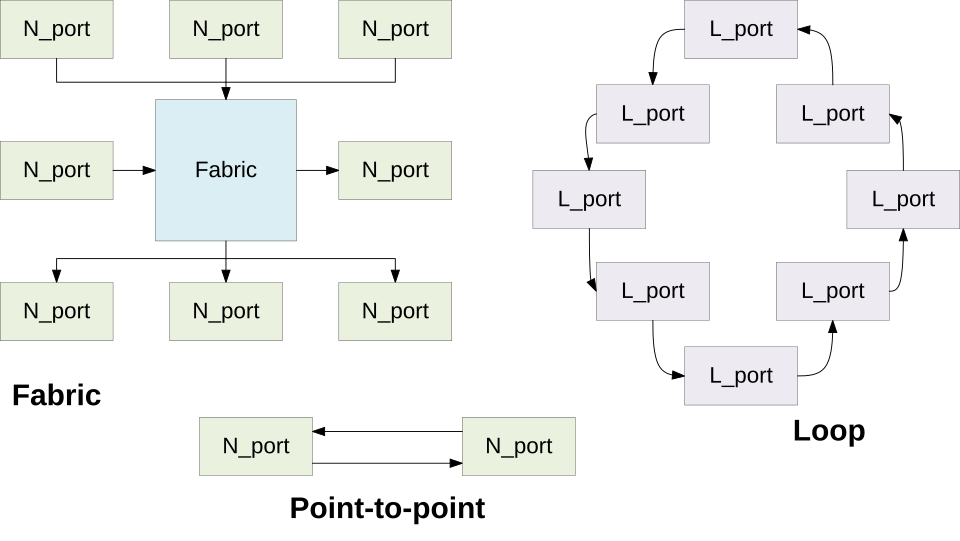
\includegraphics[width=0.6\textwidth]{img/san5.png}
	\caption{Topologia Canal de Fibra}
	\label{fig:san5}
\end{figure}

\subsubsection{Topología Punto a Punto (Point-to-Point)}

La topología punto a punto es la más simple. En esta configuración, la conexión entre dos dispositivos es dedicada y directa, sin ningún dispositivo de interconexión intermedio. Este esquema crea un ancho de banda dedicado completo entre los puntos liga dos. La ventaja principal de esta topología es la simplicidad y el ancho de banda completo dedicado disponible para la comunicación entre los dos dispositivos. Sin embargo, la desventaja significativa es la falta de escalabilidad, ya que cada par de dispositivos que necesita comunicarse requiere su propio enlace físico dedicado.

\subsubsection{Topología Arbitrated Loop (FC-AL)}

La topología Arbitrated Loop (FC-AL) es una topología en anillo que comparte el ancho de banda de Fibre Channel entre múltiples endpoints. El loop es implementado dentro de un hub que interconecta los endpoints, creando un anillo lógico donde los datos circulan pasando por cada dispositivo en el loop. La comunicación ocurre mediante un mecanismo de arbitraje donde los dispositivos deben solicitar y obtener el control del loop antes de poder transmitir datos.

FC-AL tiene limitaciones significativas: si un dispositivo en el loop falla, puede romper todo el anillo a menos que se implementen mecanismos de redundancia; el ancho de banda es compartido entre todos los dispositivos, limitando el rendimiento por dispositivo; y la latencia puede ser variable dependiendo de la posición del dispositivo en el loop y del tráfico existente.

\subsubsection{Topología Fabric Switching (FC-SW)}

La topología Fabric Switching es la topología más común y utilizada en implementaciones modernas. Utiliza uno o más switches fabric para interconectar dispositivos, proporcionando la mayor flexibilidad y haciendo el mejor uso del ancho de banda agregado mediante el uso de conexiones de conmutación entre endpoints. En una fabric, cada dispositivo se conecta a un puerto en un switch FC, y el switch gestiona las conexiones entre dispositivos, permitiendo múltiples comunicaciones simultáneas a punto a través del switch.

La ventaja principal es la capacidad de múltiples conexiones simultáneas. Mientras múltiples pares de dispositivos pueden comunicarse simultáneamente a través del switch, cada par tiene acceso al ancho de banda completo del enlace. Esto proporciona un rendimiento superior para la mayoría de las cargas de trabajo empresariales. Además, la fabric ofrece alta disponibilidad, ya que la falla de un dispositivo no afecta a otros. La topología fabric también proporciona características avanzadas como Zoning para segmentación de seguridad, gestión centralizada a través de servicios de directorio, y capacidades de extensión para conectar fabrics en diferentes ubicaciones geográficas.

\subsection{Componentes físicos de una infraestructura FC}

Una implementación de Fibre Channel incluye varios componentes físicos que trabajan en conjunto para formar la red de almacenamiento. Estos componentes pueden incluir adaptadores de bus de host, convertidores de interfaz, módulos de enlace, arrays de almacenamiento, controladores, hubs, switches, bibliotecas de cinta y cables.

\begin{figure}[H]
	\centering
	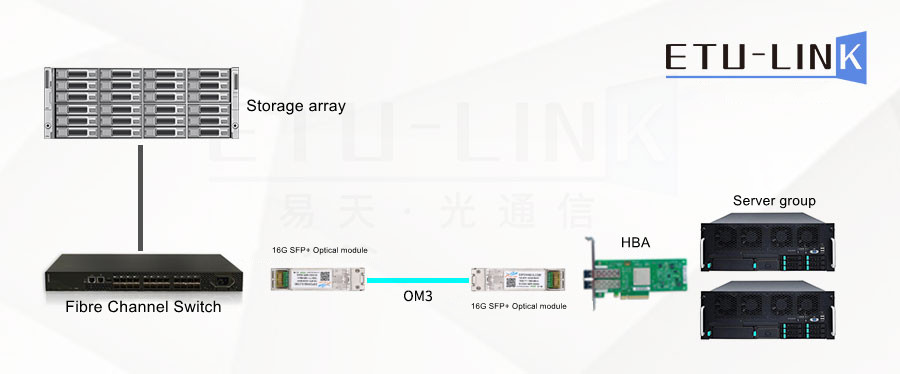
\includegraphics[width=0.6\textwidth]{img/san7.png}
	\caption{Componentes Canal de Fibra}
	\label{fig:san7}
\end{figure}

\subsubsection{HBA (Host Bus Adapter)}

Los HBA son tarjetas de interfaz especializadas instaladas en los servidores que permiten la conexión a la red Fibre Channel. Estos son hardware específicamente diseñado para comunicación de almacenamiento con procesadores que descargan del CPU principal las tareas relacionadas con el protocolo FC. Los HBAs modernos incluyen capacidades de procesamiento propio, funciones de redundancia y failover automático, y soportan velocidades de 8G, 16G, 32G y mayores. Cada HBA tiene uno o más puertos FC que se conectan a switches o directamente a dispositivos de almacenamiento.

\begin{figure}[H]
	\centering
	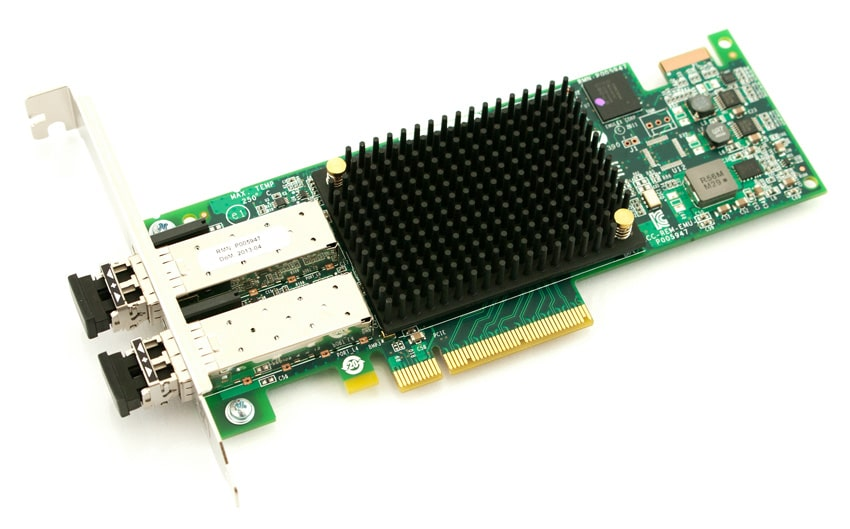
\includegraphics[width=0.4\textwidth]{img/san6.png}
	\caption{HBA}
	\label{fig:san6}
\end{figure}

\subsubsection{Switches FC}

Los switches Fibre Channel son dispositivos de interconexión especializados que forman la columna vertebral de la fabric FC. Estos switches están optimizados para manejar tráfico de E/S de almacenamiento con latencias extremadamente bajas. Cada puerto puede operar a la velocidad máxima del switch o a velocidades menores para compatibilidad con dispositivos más antiguos. Los switches incluyen funciones avanzadas como Zoning, gestión de tráfico, monitoreo de rendimiento, diagnóstico integrado, y servicios de directorio.

\begin{figure}[H]
	\centering
	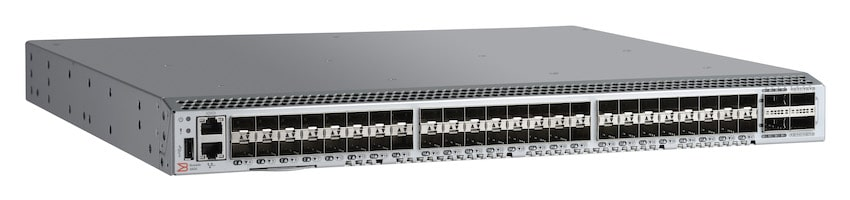
\includegraphics[width=0.6\textwidth]{img/san8.png}
	\caption{Switches FC}
	\label{fig:san8}
\end{figure}

\subsubsection{Directores FC}

Los directores FC son dispositivos de nivel empresarial que combinan características de switches con alta disponibilidad y escalabilidad extremas. A diferencia de los switches convencionales que tienen un número fijo de puertos, los directores utilizan chasis modulares con tarjetas que pueden agregarse según sea necesario. Los directores típicamente soportan cientos o miles de puertos en un solo chasis, y implementan redundancia completa incluyendo fuentes de poder duales, ventiladores redundantes, y controladores redundantes para eliminar puntos únicos de falla.

\subsubsection{Cables y Transceivers}

Los cables Fibre Channel pueden ser de fibra óptica o cobre. La fibra óptica es el medio más común, disponible en tipos principales: fibra multimodo para distancias cortas hasta varios cientos de metros, y fibra monomodo para distancias largas hasta varios kilómetros. Los transceivers (SFPs) son módulos que convierten señales eléctricas del HBA o switch a señales ópticas para transmisión por fibra, y viceversa.

\begin{figure}[H]
	\centering
	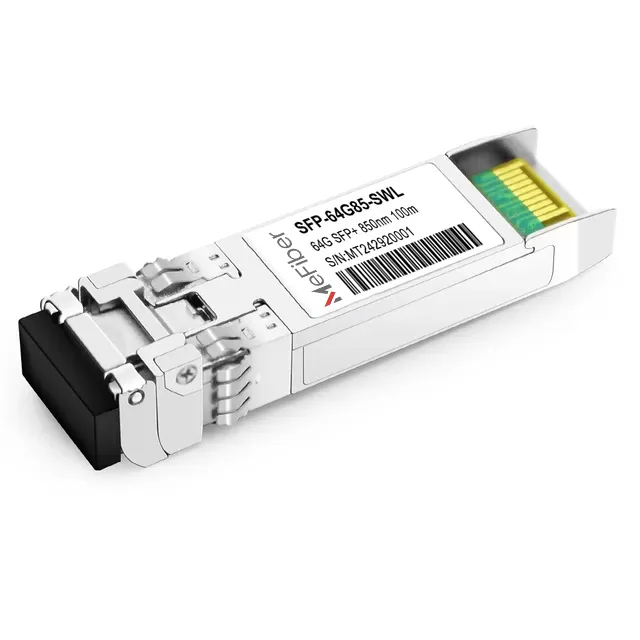
\includegraphics[width=0.4\textwidth]{img/san9.png}
	\caption{SFP}
	\label{fig:san9}
\end{figure}

\begin{figure}[H]
	\centering
	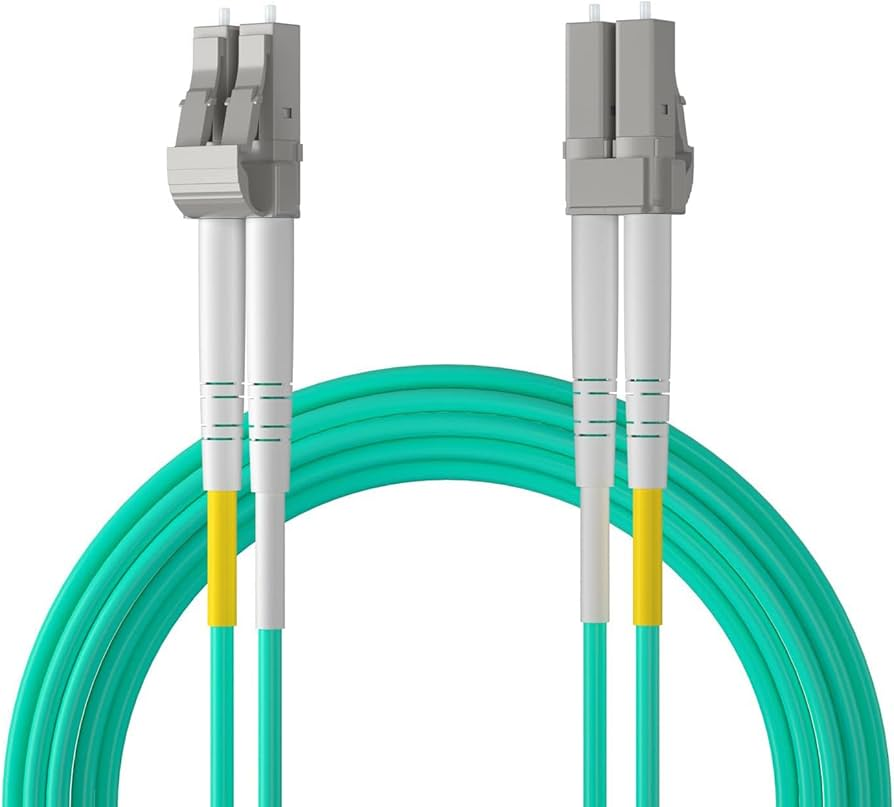
\includegraphics[width=0.4\textwidth]{img/san10.png}
	\caption{Cable FC}
	\label{fig:san10}
\end{figure}

\subsection{Zoning: Hard Zoning vs Soft Zoning como mecanismo de segmentación y seguridad}

El Zoning es un mecanismo fundamental de seguridad y segmentación en redes Fibre Channel que permite dividir una fabric en grupos lógicos de dispositivos que pueden comunicarse entre sí. Similar a las VLANs en redes Ethernet, el Zoning controla qué servidores pueden acceder a qué dispositivos de almacenamiento, proporcionando aislamiento lógico y seguridad.

\begin{figure}[H]
	\centering
	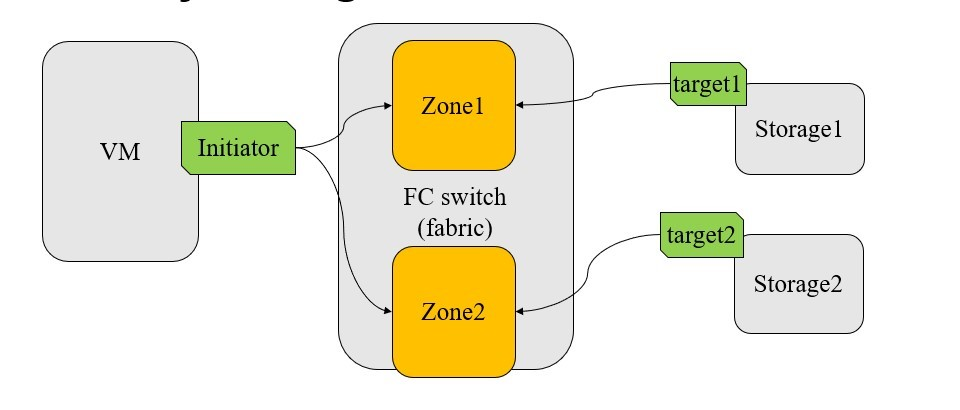
\includegraphics[width=0.6\textwidth]{img/san11.png}
	\caption{Zoning}
	\label{fig:san11}
\end{figure}

\subsubsection{Hard Zoning (Zoning por Hardware)}

El Hard Zoning se implementa a nivel de hardware en los switches FC. El zoning se basa en direcciones físicas de puerto (Port-based zoning), donde los puertos específicos del switch están asignados a zonas específicas. Solo los dispositivos conectados a puertos dentro de la misma zona pueden comunicarse entre sí. Si un dispositivo se mueve a un puerto diferente, su pertenencia a la zona cambia automáticamente basada en la configuración del puerto.

Las ventajas del Hard Zoning incluyen seguridad física: un dispositivo no puede unirse a una zona simplemente cambiando su configuración de software, ya que el acceso está determinado físicamente por el puerto al que está conectado. El hard zoning también es típicamente más eficiente en términos de rendimiento, ya que el switch puede implementar las reglas de zoning directamente en hardware. Sin embargo, la desventaja principal es la falta de flexibilidad: reorganizar zonas requiere mover físicamente los cables a diferentes puertos, lo que puede ser inconveniente en instalaciones grandes.

\subsubsection{Soft Zoning (Zoning por Software)}

El Soft Zoning se implementa a nivel de software en los switches FC. El zoning se basa en identificadores de dispositivo World Wide Name (WWN-based zoning), donde cada HBA y puerto de almacenamiento tiene un identificador único mundial emitido de fábrica. Las zonas se definen por estos WWNs independientemente del puerto físico al que está conectado el dispositivo.

Las ventajas del Soft Zoning incluyen flexibilidad significativa: los dispositivos pueden ser reorganizados en zonas simplemente cambiando la configuración del switch, sin necesidad de mover cables físicamente. Esto facilita la gestión de zonas en instalaciones grandes y dinámicas. Los WWNs son únicos globalmente, lo que previene conflictos de direccionamiento. Sin embargo, el Soft Zoning es teóricamente menos seguro que Hard Zoning, ya que un dispositivo con conocimiento técnico podría intentar falsificar un WWN.

\subsection{FCoE (Fibre Channel over Ethernet) como solución de convergencia y su relevancia actual}

Fibre Channel over Ethernet (FCoE) representa un enfoque híbrido que intenta combinar las ventajas de Fibre Channel con las ventajas de Ethernet. FCoE encapsula tramas de Fibre Channel dentro de paquetes Ethernet, permitiendo que el tráfico de Fibre Channel viaje a través de infraestructura de red Ethernet.

\begin{figure}[H]
	\centering
	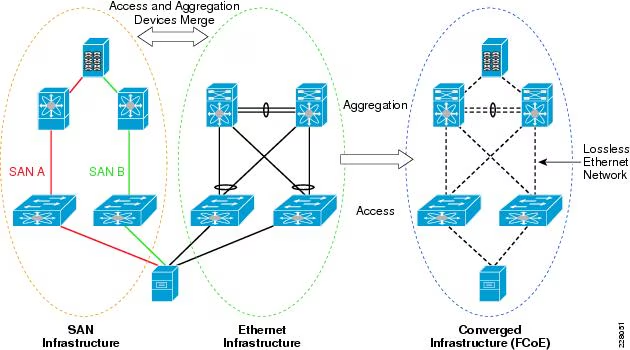
\includegraphics[width=0.7\textwidth]{img/san12.png}
	\caption{FCoE}
	\label{fig:san12}
\end{figure}

\subsubsection{Arquitectura y Funcionamiento de FCoE}

La arquitectura de FCoE requiere adaptadores de red especializados llamados Converged Network Adapters (CNA) que pueden manejar tanto tráfico de red convencional como tráfico de Fibre Channel sobre Ethernet. Estos CNAs son más costosos que las tarjetas de red Ethernet convencionales pero más económicos que los HBAs de Fibre Channel puros. Los switches requieren ser switches Ethernet que soporten FCoE, frecuentemente llamados FCoE-enabled switches o DCB (Data Center Bridging) switches. 

El objetivo principal de FCoE es consolidar las redes de almacenamiento y redes de datos en una sola infraestructura física. En lugar de mantener dos redes separadas (una LAN Ethernet y una SAN FC), FCoE permite que ambas compartan la misma infraestructura de cableado y switches. Esta consolidación reduce significativamente la cantidad de cables, puertos en servidores y dispositivos de red, simplificando el centro de datos y reduciendo costos de capital y operación.

Los administradores pueden utilizar las mismas herramientas de gestión de FC que ya conocen mientras utilizan hardware Ethernet. FCoE también puede reducir el consumo de energía y espacio en el centro de datos al reducir la cantidad de hardware. 

Sin embargo, FCoE presenta desafíos significativos. La tecnología es más compleja de implementar y gestionar, requiriendo conocimientos tanto de Fibre Channel como de Ethernet avanzado con DCB. El ecosistema de FCoE es menos maduro que los de FC e iSCSI, con menos proveedores ofreciendo productos FCoE y menos opciones de hardware. El FCoE ha encontrado adopción limitada en el mercado, ya que muchas organizaciones han optado directamente por iSCSI para redes basadas en Ethernet o han permanecido con FC tradicional para máximo rendimiento.